\documentclass[xetex,mathserif,serif]{beamer}
\usepackage{polyglossia}
\setdefaultlanguage[babelshorthands=true]{russian}
\usepackage{minted}
\usepackage{tabu}
\usepackage{forest}
\usepackage{moresize}
\usepackage{textpos}

\useoutertheme{infolines}

\usepackage{fontspec}
\setmainfont{FreeSans}
\newfontfamily{\russianfonttt}{FreeSans}

\definecolor{links}{HTML}{2A1B81}
\hypersetup{colorlinks,linkcolor=,urlcolor=links}


\tabulinesep=1.2mm

\title{GUI на WPF}
\subtitle{Часть 1}
\author[Юрий Литвинов]{Юрий Литвинов\\\small{\textcolor{gray}{yurii.litvinov@gmail.com}}}
\date{15.11.2019г}

\newcommand{\DownArrow} {
	\hspace{2cm}\begin{LARGE}$\downarrow$\end{LARGE}
}

\newcommand{\attribution}[1] {
\vspace{-5mm}\begin{flushright}\begin{scriptsize}\textcolor{gray}{\textcopyright\, #1}\end{scriptsize}\end{flushright}
}

\begin{document}

	\frame{\titlepage}

	\section{Введение}

	\begin{frame}
		\frametitle{Windows Presentation Foundation}
		\begin{itemize}
			\item Появилась в .NET 3.0, как альтернатива WinForms
			\begin{itemize}
				\item Использует DirectX для отображения контролов
			\end{itemize}
			\item Отделение разметки пользовательского интерфейса от кода --- язык XAML (eXtensible Application Markup Language)
			\begin{itemize}
				\item Специальная среда разработки --- Microsoft Blend
			\end{itemize}
			\item Несколько ``веток'' WPF --- Silverlight, Windows Runtime XAML Framework
			\item Архитектурно сильно отличается от WinForms, несколько сложнее в изучении
			\begin{itemize}
				\item Data binding
				\begin{itemize}
					\item Паттерн Model-View-Viewmodel (MVVM)
				\end{itemize}
				\item Templates (Styles)
				\item Resources
			\end{itemize}
		\end{itemize}
	\end{frame}

	\section{Синтаксис XAML}

	\begin{frame}[fragile]
		\frametitle{XAML}
		\framesubtitle{eXtensible Application Markup Language}
		\begin{itemize}
			\item На самом деле, язык описания правил создания и инициализации произвольных объектов
			\begin{itemize}
				\item Есть отдельный XAML-парсер, позволяющий создавать дерево объектов по XAML-описанию
				\item Не путать с JSON и механизмами сериализации
			\end{itemize}
			\item Базируется на XML
			\begin{itemize}
				\item Тэги, атрибуты, пространства имён
			\end{itemize}
		\end{itemize}

		XAML:
		\begin{footnotesize}
			\begin{minted}{xml}
<Button xmlns="http://schemas.microsoft.com/winfx/2006/xaml/presentation"
    Content="OK" />
			\end{minted}
		\end{footnotesize}

		C\#:
		\begin{footnotesize}
			\begin{minted}{csharp}
System.Windows.Controls.Button b = new System.Windows.Controls.Button();
b.Content = "OK";
			\end{minted}
		\end{footnotesize}
	\end{frame}

	\begin{frame}[fragile]
		\frametitle{``Полная форма'' записи атрибутов}
		\begin{footnotesize}
			\begin{minted}{xml}
<Button xmlns="http://schemas.microsoft.com/winfx/2006/xaml/presentation">
    <Button.Content>
        <Rectangle Height="40" Width="40" Fill="Black" />
    </Button.Content>
</Button>
			\end{minted}
		\end{footnotesize}

		\DownArrow
		\begin{footnotesize}
			\begin{minted}{csharp}
System.Windows.Controls.Button b = new System.Windows.Controls.Button();
System.Windows.Shapes.Rectangle r = new System.Windows.Shapes.Rectangle();
r.Width = 40;
r.Height = 40;
r.Fill = System.Windows.Media.Brushes.Black;
b.Content = r;
			\end{minted}
		\end{footnotesize}
	\end{frame}

	\begin{frame}[fragile]
		\frametitle{Конвертеры типов}
		\begin{footnotesize}
			\begin{minted}{xml}
<Button xmlns="http://schemas.microsoft.com/winfx/2006/xaml/presentation"
    Content="OK" Background="White" />
			\end{minted}
		\end{footnotesize}

		\DownArrow
		\begin{footnotesize}
			\begin{minted}{csharp}
System.Windows.Controls.Button b = new System.Windows.Controls.Button();
b.Content = "OK";
b.Background = System.Windows.Media.Brushes.White;
			\end{minted}
		\end{footnotesize}

		\DownArrow
		\begin{footnotesize}
			\begin{minted}{xml}
<Button xmlns="http://schemas.microsoft.com/winfx/2006/xaml/presentation"
    Content="OK" />
    <Button.Background>
        <SolidColorBrush Color="White" />
    </Button.Background>
</Button>
			\end{minted}
		\end{footnotesize}
	\end{frame}

	\begin{frame}[fragile]
		\frametitle{Расширения}
		\begin{itemize}
			\item Похожи на конвертеры
			\begin{itemize}
				\item Возможность вызывать произвольный код в процессе создания объекта
			\end{itemize}
			\item Есть куча встроенных расширений, можно писать свои
		\end{itemize}
		\begin{footnotesize}
			\begin{minted}{xml}
<Button xmlns="http://schemas.microsoft.com/winfx/2006/xaml/presentation"
    xmlns:x="http://schemas.microsoft.com/winfx/2006/xaml"
    Background="{x:Null}"
    Height="{x:Static SystemParameters.IconHeight}"
    Content="{Binding Path=Height, RelativeSource={RelativeSource Self}}" />
			\end{minted}
		\end{footnotesize}
	\end{frame}

	\begin{frame}[fragile]
		\frametitle{Дети элементов}
		\begin{itemize}
			\item Content
			\item Элементы коллекции
			\item Результат вызова конвертеров
		\end{itemize}
		\vspace{3mm}
		\begin{scriptsize}
			\begin{minted}{xml}
<Button xmlns="http://schemas.microsoft.com/winfx/2006/xaml/presentation">
    <Button.Content>
        <Rectangle Height="40" Width="40" Fill="Black" />
    </Button.Content>
</Button>
			\end{minted}

			\DownArrow
			\begin{minted}{xml}
<Button xmlns="http://schemas.microsoft.com/winfx/2006/xaml/presentation">
    <Rectangle Height="40" Width="40" Fill="Black" />
</Button>
			\end{minted}
		\end{scriptsize}
	\end{frame}

	\begin{frame}[fragile]
		\frametitle{Коллекции}
		\begin{scriptsize}
			\begin{itemize}
				\item Списки
					\begin{minted}{xml}
<ListBox xmlns="http://schemas.microsoft.com/winfx/2006/xaml/presentation">
    <ListBox.Items>
        <ListBoxItem Content="Item 1" />
        <ListBoxItem Content="Item 2" />
    </ListBox.Items>
</ListBox>
					\end{minted}
				\item Словари
					\begin{minted}{xml}
<ResourceDictionary xmlns="http://schemas.microsoft.com/winfx/2006/xaml/presentation"
        xmlns:x="http://schemas.microsoft.com/winfx/2006/xaml">
    <Color x:Key="1" A="255" R="255" G="255" B="255" />
    <Color x:Key="2" A="0" R="0" G="0" B="0" />
</ResourceDictionary>
					\end{minted}
			\end{itemize}
		\end{scriptsize}
	\end{frame}

	\section{Архитектура WPF}

	\begin{frame}[fragile]
		\frametitle{Структура классов WPF}
		\begin{columns}
			\begin{column}{0.7\textwidth}
				\begin{itemize}
					\item DispatcherObject --- потоки и сообщения
					\item DependencyObject --- продвинутая работа со свойствами
					\item Visual --- общение с движком рисования
					\item UIElement --- лейаут, события
					\item FrameworkElement --- ещё лейаут, стили
					\item Control --- шаблоны
				\end{itemize}
			\end{column}
			\begin{column}{0.3\textwidth}
				\begin{center}
					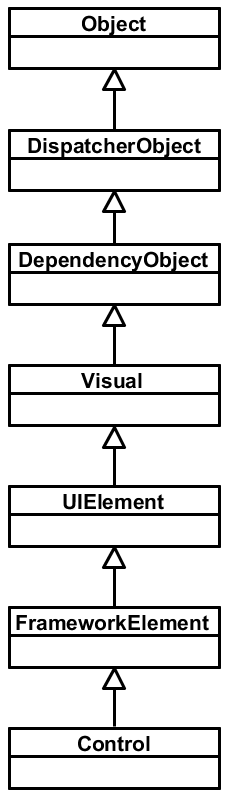
\includegraphics[width=0.5\textwidth]{wpfClassStructure.png}
				\end{center}
			\end{column}
		\end{columns}
	\end{frame}

	\begin{frame}
		\frametitle{Логическое дерево}
		\begin{columns}
			\begin{column}{0.5\textwidth}
				\begin{center}
					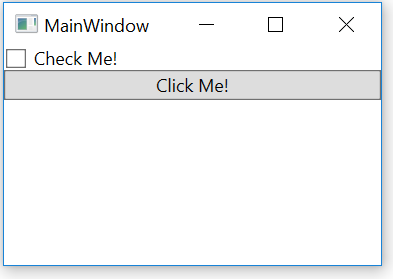
\includegraphics[width=0.6\textwidth]{wpfApp.png}
				\end{center}
			\end{column}
			\begin{column}{0.5\textwidth}
				\begin{center}
					\begin{tiny}
						\begin{forest}
							for tree={rectangle,draw}
							[MainWindow
								[StackPanel
									[CheckBox
										[String]
									]
									[Button
										[String]
									]
								]
							]
						\end{forest}
					\end{tiny}
				\end{center}
			\end{column}
		\end{columns}
	\end{frame}

	\begin{frame}
		\frametitle{Визуальное дерево}
		\begin{columns}
			\begin{column}{0.4\textwidth}
				\begin{center}
					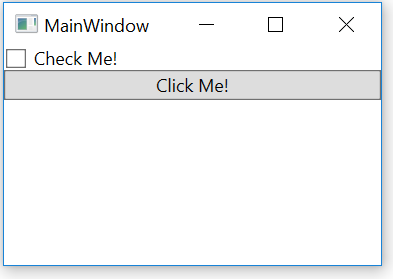
\includegraphics[width=0.6\textwidth]{wpfApp.png}
				\end{center}
			\end{column}
			\begin{column}{0.6\textwidth}
				\begin{tiny}
					\begin{forest}
						for tree={rectangle,draw,align=center}
						[MainWindow
							[Border
								[AdornerDecorator
									[ContentPresenter
										[StackPanel
											[CheckBox
												[TemplateRoot
													[checkBoxBorder
														[MarkGrid
															[optionMark]
															[indeterminateMark]
														]
													]
													[contentPresenter
														[TextBlock]
													]
												]
											]
											[Button
												[border
													[contentPresenter
														[TextBlock]
													]
												]
											]
										]
									]
								]
							]
						]
					\end{forest}
				\end{tiny}
			\end{column}
		\end{columns}
	\end{frame}

	\section{Зависимые свойства}

	\begin{frame}
		\frametitle{Dependency Properties}
		\begin{itemize}
			\item \textit{Зависят} от ``провайдеров'', на основании которых они вычисляют своё текущее значение
			\item Похожи на обычные свойства, но:
			\begin{itemize}
				\item Обеспечивают оповещение об изменениях
				\item Позволяют наследовать значения свойств от предка в логическом дереве
				\item Позволяют добавлять объекту свойства, которых у него не было
			\end{itemize}
			\item Реализуются как обычные свойства с некоторой дополнительной машинерией, которая прячет за собой хеш-таблицу
			\item Нужны, чтобы можно было легко менять свойства, делать анимацию и подобного рода вещи прямо из XAML-а
			\begin{itemize}
				\item Декларативность и Data-Driven Development --- базовые принципы архитектуры WPF
			\end{itemize}
		\end{itemize}
	\end{frame}

	\begin{frame}[fragile]
		\frametitle{Пример реализации зависимого свойства}
		\begin{tiny}
			\begin{minted}{csharp}
public class Button: ButtonBase
{
    public static readonly DependencyProperty IsDefaultProperty;

    static Button()
    {
        Button.IsDefaultProperty = DependencyProperty.Register(
            "IsDefault",
            typeof(bool),
            typeof(Button),
            new FrameworkPropertyMetadata(
                false, 
                new PropertyChangedCallback(OnIsDefaultChanged)
                )
            );
    }

    public bool IsDefault
    {
        get => (bool) GetValue(Button.IsDefaultProperty);
        set => SetValue(Button.IsDefaultProperty, value);
    }

    private static void OnIsDefaultChanged(DependencyObject o, 
        DependencyPropertyChangedEventArgs e)
    {
        ...
    }
}
			\end{minted}
		\end{tiny}
	\end{frame}

	\begin{frame}[fragile]
		\frametitle{Порядок вычисления зависимых свойств}
		\begin{columns}
			\begin{column}{0.5\textwidth}
				\begin{enumerate}
					\item Локальное значение
					\item Триггер шаблона родителя
					\item Шаблон родителя
					\item Триггеры стиля
					\item Триггеры шаблона
					\item Сеттеры стиля
					\item Триггеры темы
					\item Сеттеры темы
					\item Унаследованное значение
					\item Значение по умолчанию
				\end{enumerate}
			\end{column}
			\begin{column}{0.5\textwidth}
				\begin{footnotesize}
					\begin{forest}
						for tree={rectangle,draw,align=center,edge=->,fill=blue!80!darkgray!25,rounded corners}
						[Определение базового значения
							[Вычисление (если выражение)
								[Применение анимации
									[Приведение
										[Валидация]
									]
								]
							]
						]
					\end{forest}
				\end{footnotesize}
			\end{column}
		\end{columns}
	\end{frame}

	\begin{frame}[fragile]
		\frametitle{Пример триггера стиля}
		\begin{minted}{xml}
<Button Content="Click Me!">
    <Button.Style>
        <Style TargetType="{x:Type Button}">
            <Style.Triggers>
                <Trigger Property="IsMouseOver" Value="True">
                    <Setter Property="Foreground" Value="Blue"/>
                </Trigger>
            </Style.Triggers>
        </Style>
    </Button.Style>
</Button>
		\end{minted}
	\end{frame}

	\begin{frame}[fragile]
		\frametitle{Attached Properties}
		\begin{small}
			\begin{minted}{xml}
<StackPanel TextElement.FontSize="30" TextElement.FontStyle="Italic">
    <CheckBox Content="Check Me!"/>
    <Button Content="Click Me!"/>
</StackPanel>
			\end{minted}
		\end{small}
		\begin{center}\begin{LARGE}$\downarrow$\end{LARGE}\end{center}
		\begin{center}
			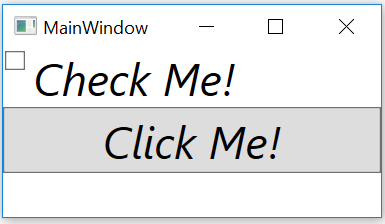
\includegraphics[width=0.3\textwidth]{fancyWindow.png}
		\end{center}
	\end{frame}

	\section{Маршрутизируемые события}
	
	\begin{frame}[fragile]
		\frametitle{Routed Events}
		\begin{scriptsize}
			\begin{minted}{csharp}
public class Button : ButtonBase
{
    public static readonly RoutedEvent ClickEvent;

    static Button()
    {
        Button.ClickEvent = EventManager.RegisterRoutedEvent("Click",
            RoutingStrategy.Bubble, typeof(RoutedEventHandler), typeof(Button));
    }

    public event RoutedEventHandler Click
    {
        add { AddHandler(Button.ClickEvent, value); }
        remove { RemoveHandler(Button.ClickEvent, value); }
    }

    protected override void OnMouseLeftButtonDown(MouseButtonEventArgs e)
    {
        RaiseEvent(new RoutedEventArgs(Button.ClickEvent, this));
    }
    ...
}
			\end{minted}
		\end{scriptsize}
	\end{frame}

	\begin{frame}
		\frametitle{Routed Events, события}
		\begin{itemize}
			\item Стратегии маршрутизации:
			\begin{itemize}
				\item \textbf{Bubbling} --- снизу вверх
				\begin{itemize}
					\item Контролы в WPF по соглашению реагируют только на них
				\end{itemize}
				\item \textbf{Tunneling} --- сверху вниз
				\begin{itemize}
					\item По соглашению имеют префикс Preview и парное Bubbling-событие
				\end{itemize}
				\item \textbf{Direct} --- как обычные события в C\#
			\end{itemize}
			\item RoutedEventArgs:
			\begin{itemize}
				\item \textbf{Source} --- элемент логического дерева
				\item \textbf{OriginalSource} --- элемент визуального дерева
				\item \textbf{Handled} --- заканчивает распространение события
				\begin{itemize}
					\item На самом деле, нет, можно подписаться и на обработанное
					\item Обработка PreviewX отменяет и bubbling-событие X
				\end{itemize}
			\end{itemize}
		\end{itemize}
	\end{frame}

	\section{Data Binding}

	\begin{frame}[fragile]
		\frametitle{Подробнее про Data Binding}
		\begin{footnotesize}
			\begin{minted}{csharp}
void treeView_SelectedItemChanged(object sender,
    RoutedPropertyChangedEventArgs<object> e)
{
    currentFolder.Text = (treeView.SelectedItem as TreeViewItem).Header.ToString();
    Refresh();
}
			\end{minted}
		\end{footnotesize}
		\DownArrow
		\begin{footnotesize}
			\begin{minted}{csharp}
public MainWindow()
{
    InitializeComponent();
    Binding binding = new Binding();
    binding.Source = treeView;
    binding.Path = new PropertyPath("SelectedItem.Header");
    currentFolder.SetBinding(TextBlock.TextProperty, binding);
}
			\end{minted}
		\end{footnotesize}
	\end{frame}

	\begin{frame}[fragile]
		\frametitle{То же в XAML}
		\begin{footnotesize}
			\begin{minted}{csharp}
public MainWindow()
{
    InitializeComponent();
    Binding binding = new Binding();
    binding.Source = treeView;
    binding.Path = new PropertyPath("SelectedItem.Header");
    currentFolder.SetBinding(TextBlock.TextProperty, binding);
}
			\end{minted}
		\end{footnotesize}
		\DownArrow
		\begin{footnotesize}
			\begin{minted}{xml}
<TextBlock x:Name="currentFolder" DockPanel.Dock="Top"
    Text="{Binding ElementName=treeView, Path=SelectedItem.Header}"
    Background="AliceBlue" FontSize="16" />
			\end{minted}
		\end{footnotesize}
	\end{frame}

	\begin{frame}[fragile]
		\frametitle{Привязка к ``обычным'' свойствам}
		\begin{footnotesize}
			\begin{minted}{xml}
<Label x:Name="numItemsLabel"
    Content="{Binding Source={StaticResource photos}, Path=Count}"
    DockPanel.Dock="Bottom"/>
			\end{minted}
		\end{footnotesize}
		Так оно не будет обновляться, надо, чтобы:
		\begin{itemize}
			\item был реализован INotifyPropertyChanged
			\item было событие XXXChanged, где XXX --- имя свойства
			\item для коллекций --- ObservableCollection
		\end{itemize}
		Target --- всегда DependencyProperty
	\end{frame}

	\begin{frame}[fragile]
		\frametitle{Привязка ``составных'' контролов к коллекциям}
		\begin{footnotesize}
			\begin{minted}{xml}
<ListBox x:Name="pictureBox" DisplayMemberPath="Name"
    ItemsSource="{Binding Source={StaticResource photos}}" ...>
    ...
</ListBox>
			\end{minted}
		\end{footnotesize}
		\DownArrow
		\begin{footnotesize}
			\begin{minted}{xml}
<ListBox x:Name="pictureBox"
    ItemsSource="{Binding Source={StaticResource photos}}" ...>
    <ListBox.ItemTemplate>
        <DataTemplate>
            <Image Source="{Binding Path=FullPath}" Height="35"/>
        </DataTemplate>
    </ListBox.ItemTemplate>
    ...
</ListBox>
			\end{minted}
		\end{footnotesize}
	\end{frame}

	\begin{frame}[fragile]
		\frametitle{DataContext}
		\begin{footnotesize}
			\begin{minted}{xml}
<StackPanel DataContext="{StaticResource photos}">
    <Label x:Name="numItemsLabel"
        Content="{Binding Path=Count}" .../>
    ...
    <ListBox x:Name="pictureBox" DisplayMemberPath="Name"
        ItemsSource="{Binding}" ...>
        ...
    </ListBox>
    ...
</StackPanel>
			\end{minted}
		\end{footnotesize}
	\end{frame}

	\begin{frame}[fragile]
		\frametitle{Конвертеры}
		\begin{ssmall}
			\begin{minted}{xml}
<Window.Resources>
    <local:CountToBackgroundConverter x:Key="myConverter"/>
</Window.Resources>
...
<Label Background="{Binding Path=Count, Converter={StaticResource myConverter},
    Source={StaticResource photos}}" .../>
			\end{minted}
			\vspace{3mm}
			\begin{minted}{csharp}
public class CountToBackgroundConverter : IValueConverter
{
    public object Convert(object value, Type targetType, object parameter,
        CultureInfo culture)
    {
        if (targetType != typeof(Brush))
            throw new InvalidOperationException("The target must be a Brush!");
        int num = int.Parse(value.ToString());
        return (num == 0 ? Brushes.Yellow : Brushes.Transparent);
    }

    public object ConvertBack(object value, Type targetType, object parameter,
        CultureInfo culture)
    {
        return DependencyProperty.UnsetValue;
    }
}
			\end{minted}
		\end{ssmall}
	\end{frame}

	\begin{frame}
		\frametitle{Направления привязки}
		\begin{itemize}
			\item OneWay --- то, что мы делали до этого
			\begin{itemize}
				\item По умолчанию для большинства свойств
			\end{itemize}
			\item TwoWay --- в обе стороны, для редактируемых контролов
			\begin{itemize}
				\item По умолчанию для, например, TextBox.Text
				\item UpdateSourceTrigger --- PropertyChanged, LostFocus, Explicit
			\end{itemize}
			\item OneWayToSource --- от цели к источнику, для полей ввода
			\item OneTime --- без нотификаций об изменении вовсе
		\end{itemize}
	\end{frame}

	\begin{frame}
		\frametitle{Паттерн ``Model-View-View Model''}
		\begin{center}
			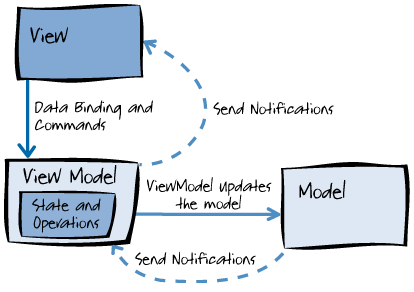
\includegraphics[width=0.5\textwidth]{mvvm.png}
		\end{center}
		\attribution{https://msdn.microsoft.com/en-us/library/hh848246.aspx}
	\end{frame}

	\section{Геометрия}

	\begin{frame}
		\frametitle{Геометрия контрола}
		\begin{center}
			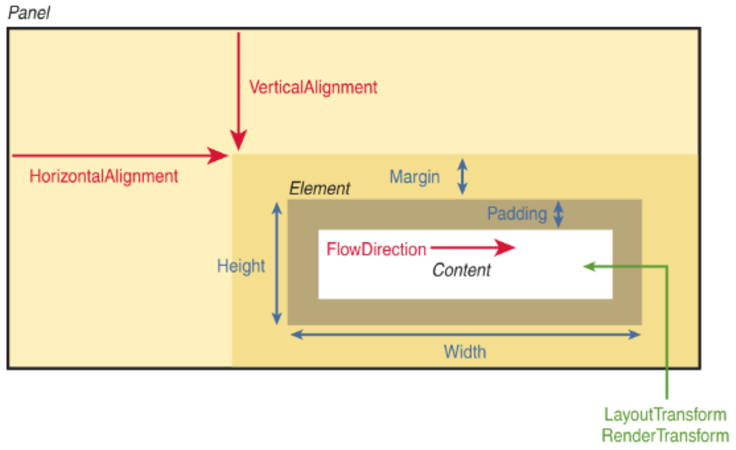
\includegraphics[width=0.5\textwidth]{controlGeometry.png}
		\end{center}
		\attribution{Из книги Adam Nathan, WPF 4.5 Unleashed.}
	\end{frame}

	\begin{frame}
		\frametitle{Управление положением элемента}
		\begin{columns}
			\begin{column}{0.7\textwidth}
				\begin{itemize}
					\item Абсолютное
					\begin{itemize}
						\item Padding
						\item Margin
						\item Тип System.Windows.Thickness
					\end{itemize}
					\item Выравнивание внутри родителя
					\begin{itemize}
						\item HorizontalAlignment, VerticalAlignment
						\item HorizontalContentAlignment, VerticalContentAlignment
					\end{itemize}
				\end{itemize}
			\end{column}
			\begin{column}{0.3\textwidth}
				\begin{center}
					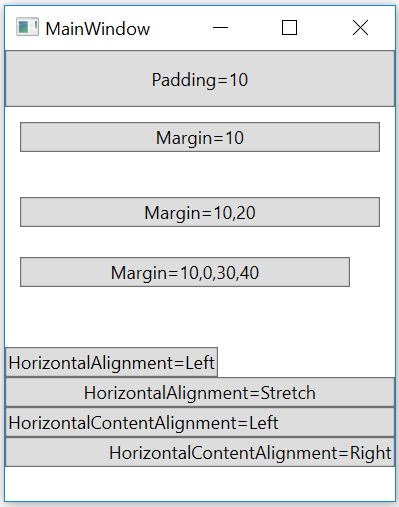
\includegraphics[width=0.9\textwidth]{geometryTest.png}
				\end{center}
			\end{column}
		\end{columns}
	\end{frame}

	\begin{frame}[fragile]
		\frametitle{Преобразования системы координат}
		\begin{columns}
			\begin{column}{0.5\textwidth}
				\begin{tiny}
					\begin{minted}{xml}
<StackPanel>
    <Button Content="Button1" Background="LightBlue"/>
    <Button Content="Button2" Background="LightGreen" >
        <Button.LayoutTransform>
            <RotateTransform Angle="45"/>
        </Button.LayoutTransform>
    </Button>
    <Button Content="Button3" Background="LightCoral"/>
</StackPanel>
					\end{minted}
				\end{tiny}

				\DownArrow
				\begin{center}
					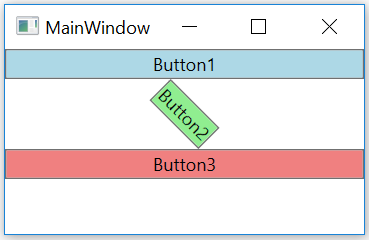
\includegraphics[width=0.6\textwidth]{layoutTransform.png}
				\end{center}
			\end{column}
			\begin{column}{0.5\textwidth}
				\begin{tiny}
					\begin{minted}{xml}
<StackPanel>
    <Button Content="Button1" Background="LightBlue"/>
    <Button Content="Button2" Background="LightGreen" >
        <Button.RenderTransform>
            <RotateTransform Angle="45"/>
        </Button.RenderTransform>
    </Button>
    <Button Content="Button3" Background="LightCoral"/>
</StackPanel>
					\end{minted}
				\end{tiny}

				\DownArrow
				\begin{center}
					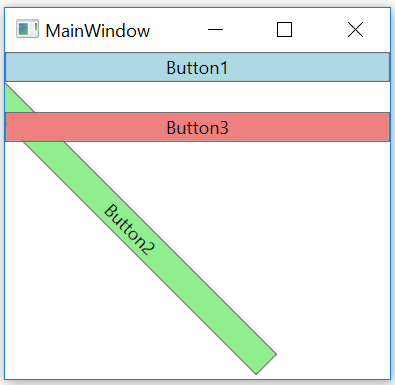
\includegraphics[width=0.6\textwidth]{renderTransform.png}
				\end{center}
			\end{column}
		\end{columns}
	\end{frame}

	\section{Заключение}
	
	\begin{frame}
		\frametitle{Литература}
		\begin{columns}
			\begin{column}{0.7\textwidth}
				Adam Nathan, WPF 4.5 Unleashed. Sams Publishing, 2013. 864pp.
				\vspace{3cm}
			\end{column}
			\begin{column}{0.3\textwidth}
				\begin{center}
					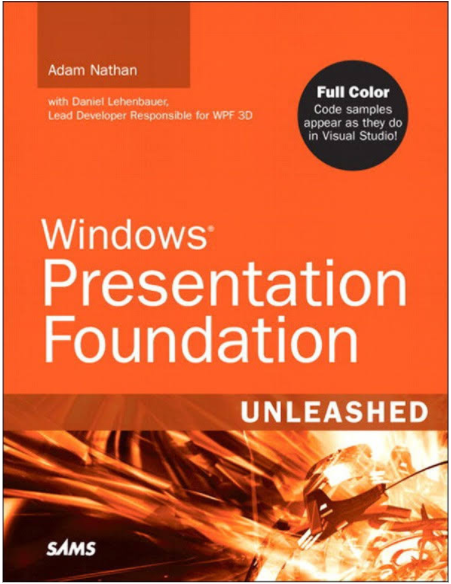
\includegraphics[width=\textwidth]{wpfBookCover.png}
				\end{center}
			\end{column}
		\end{columns}
	\end{frame}

\end{document}
